%
%  proposta
%
%  Created by Ricardo de Cillo on 2012-05-27.
%  Copyright (c) 2012 __MyCompanyName__. All rights reserved.
%
\documentclass[a4paper,11pt]{article}

% Use utf-8 encoding for foreign characters
\usepackage[brazil]{babel}
\usepackage[utf8]{inputenc}
\usepackage[T1]{fontenc}

% Setup for fullpage use
\usepackage{fullpage}

% Uncomment some of the following if you use the features
%
% Running Headers and footers
%\usepackage{fancyhdr}

% Multipart figures
%\usepackage{subfigure}

% More symbols
%\usepackage{amsmath}
%\usepackage{amssymb}
%\usepackage{latexsym}

% Surround parts of graphics with box
\usepackage{boxedminipage}

% Package for including code in the document
\usepackage{listings}

% If you want to generate a toc for each chapter (use with book)
\usepackage{minitoc}

% This is now the recommended way for checking for PDFLaTeX:
\usepackage{ifpdf}

%\newif\ifpdf
%\ifx\pdfoutput\undefined
%\pdffalse % we are not running PDFLaTeX
%\else
%\pdfoutput=1 % we are running PDFLaTeX
%\pdftrue
%\fi

\ifpdf
\usepackage[pdftex]{graphicx}
\else
\usepackage{graphicx}
\fi


\title{Proposta de monografia \\ Aplicação de análise morfológica para segmentação de páginas em imagens de documentos}
\author{ Aluno: Ricardo de Cillo \\ Supervisora: Nina S. T. Hirata }

\date{2012-05-27}

\begin{document}


\maketitle


\begin{abstract}
	Uma das aplicações da teoria de visão computacional é a análise de imagens de documentos. O objetivo desta aplicação é extrair informações sobre o conteúdo e estrutura de um documento digitalizado. Uma das etapas envolvidas é a segmentação de página que consiste na identificação de áreas da imagem correspondentes à elementos estruturais, tais como títulos, legendas e blocos de texto. Nesta monografia iremos explorar métodos morfológicos aplicados à segmentação de páginas. A qualidade da solução obtida será medida e comparada, segundo os mesmo critérios aplicados à resultados considerados estado da arte por pesquisadores da .
\end{abstract}

\section{Escopo do trabalho}

A analise de imagens de documentos, ou apenas análise de documentos, é um campo de pesquisa ativo apesar de ter sido bastante explorado nas últimas décadas. Isto se deve a sua importância prática e a complexidade dos problemas abordados. Delimitamos o escopo deste trabalho à análise de layout, como indicado no diagrama \ref{fig:context1} adaptado de \cite{Kasturi_OGorman_Govindaraju_2002}.

Para se extrair o texto de um documento cujo layout possui elementos estruturais complexos como colunas, por exemplo, precisamos primeiramente identificar estas regiões antes de aplicar um OCR.

\begin{figure}[htb!]
\begin{center}
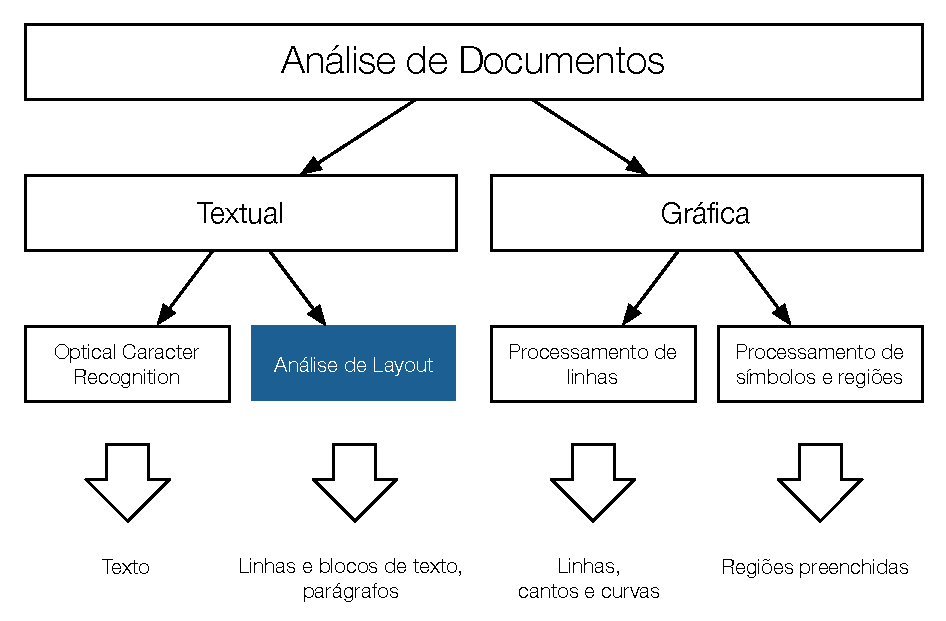
\includegraphics{assets/document_processing_areas_hierarquies.pdf}
\end{center}
\caption{Contextualização do tema do trabalho entre as áreas da análise de documentos.}
\label{fig:context1}
\end{figure}

\section{Objetivo}

Construir um software que receba como entrada a imagem de um documento digitalizado e produza como saída uma descrição geométrica \cite{10.1109/ICDAR.2007.207} de suas regiões de texto.

\section{Estrutura da monografia}

A estrutura esperada da monografia será de acordo com o esquema abaixo:

\begin{enumerate}
	\item Descrição do problema e objetivos: definição formal e exemplos.
	\item Revisão bibliográfica: resumo dos artigos estudados e trabalho importantes no assunto.
	\item Metodologia: fundamentação teórica para construção da solução.
	\item Implementação: documentação dos pontos principais da implementação.
	\item Resultados experimentais: o que deu certo ou errado e porque.
\end{enumerate}


\section{Atividades realizadas}

Até o momento eu li artigos \cite{10.1109/ICDAR.2007.207} \cite{Antonacopoulos95representationand} \cite{Antonacopoulos09arealistic} \cite{Moll07documentcontent}
\cite{Smith:2009:HPL:1634930.1635410} \cite{DBLP:conf/icdar/2009} \cite{DBLP:conf/icdar/AntonacopoulosPBP09}, estudei conceitos de visão na disciplina MAC0417 com o professor Junior Barreira, obtive um dataset para testes.

\section{Cronograma}

Vide figura \ref{fig:schedule1}.

\begin{figure}[htb!]
\begin{center}
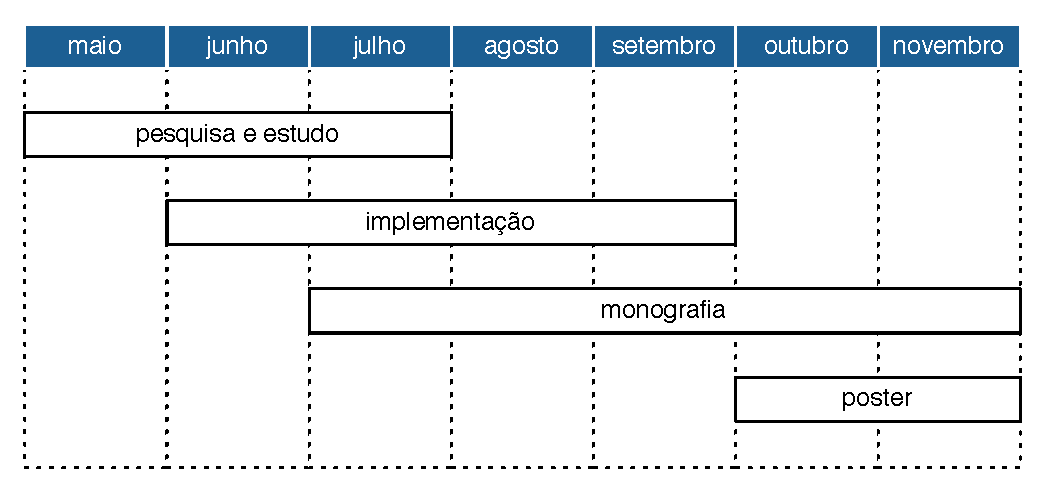
\includegraphics{assets/schedule.pdf}
\end{center}
\caption{Cronograma.}
\label{fig:schedule1}
\end{figure}

\bibliographystyle{plain}	% (uses file "plain.bst")
\bibliography{myrefs}		% expects file "myrefs.bib"

\end{document}
